\documentclass[12pt]{article}
\usepackage{fontspec}   %加這個就可以設定字體
\usepackage{xeCJK}       %讓中英文字體分開設置
\setmainfont{Times New Roman}
\setCJKmainfont{標楷體} %設定中文為系統上的字型,而英文不去更動,使用原TeX字型
\XeTeXlinebreaklocale "zh"             %這兩行一定要加,中文才能自動換行
\XeTeXlinebreakskip = 0pt plus 1pt     %這兩行一定要加,中文才能自動換行
\usepackage{amsmath, amsthm, amssymb} %引入數學符號的套件,例如實數R、定理Thm...
\usepackage{graphicx}                 %現在, 假設我們要插入 pic.png 這個圖檔, 使用
%\title{我是標題}
%\author{我是作者}
%\date{} %不要日期

\newcommand{\uA}       {\mbox{\boldmath$A$}}
\usepackage{textcomp}
\usepackage{array}
\usepackage{graphicx}
\usepackage{colortbl}
\usepackage{color,xcolor}
\usepackage{listings}
\usepackage{array,booktabs}   %這三個為表格使用的套件
\usepackage{textpos}
\usepackage{float}
\usepackage{listings}

\title{Statistical learning assignment 1 - chapter 2}
\author{孫浩哲 \hspace{0.7cm} M072040002}
\date{September 20, 2018}
\begin{document}
\maketitle
%%%%%%%%%%%%%%%%%%%%%%%%%%%%%%%%%%%%%%%%%%%%%%%%%%
\Large{8.}
\begin{itemize}
\item[a.]
\begin{verbatim}
setwd("C:/Users/asus/Desktop")
college=read.csv("college.csv")
\end{verbatim}
\item[b.]
\begin{verbatim}
rownames(college)=college[,1]
fix(college)
college=college[,-1]
fix(college)
\end{verbatim}
\item[c.]
\ \\[0.5ex]
i.\begin{verbatim}
summary(college)
\end{verbatim}
\ \\[50ex]
ii.\\[2ex]
\centerline{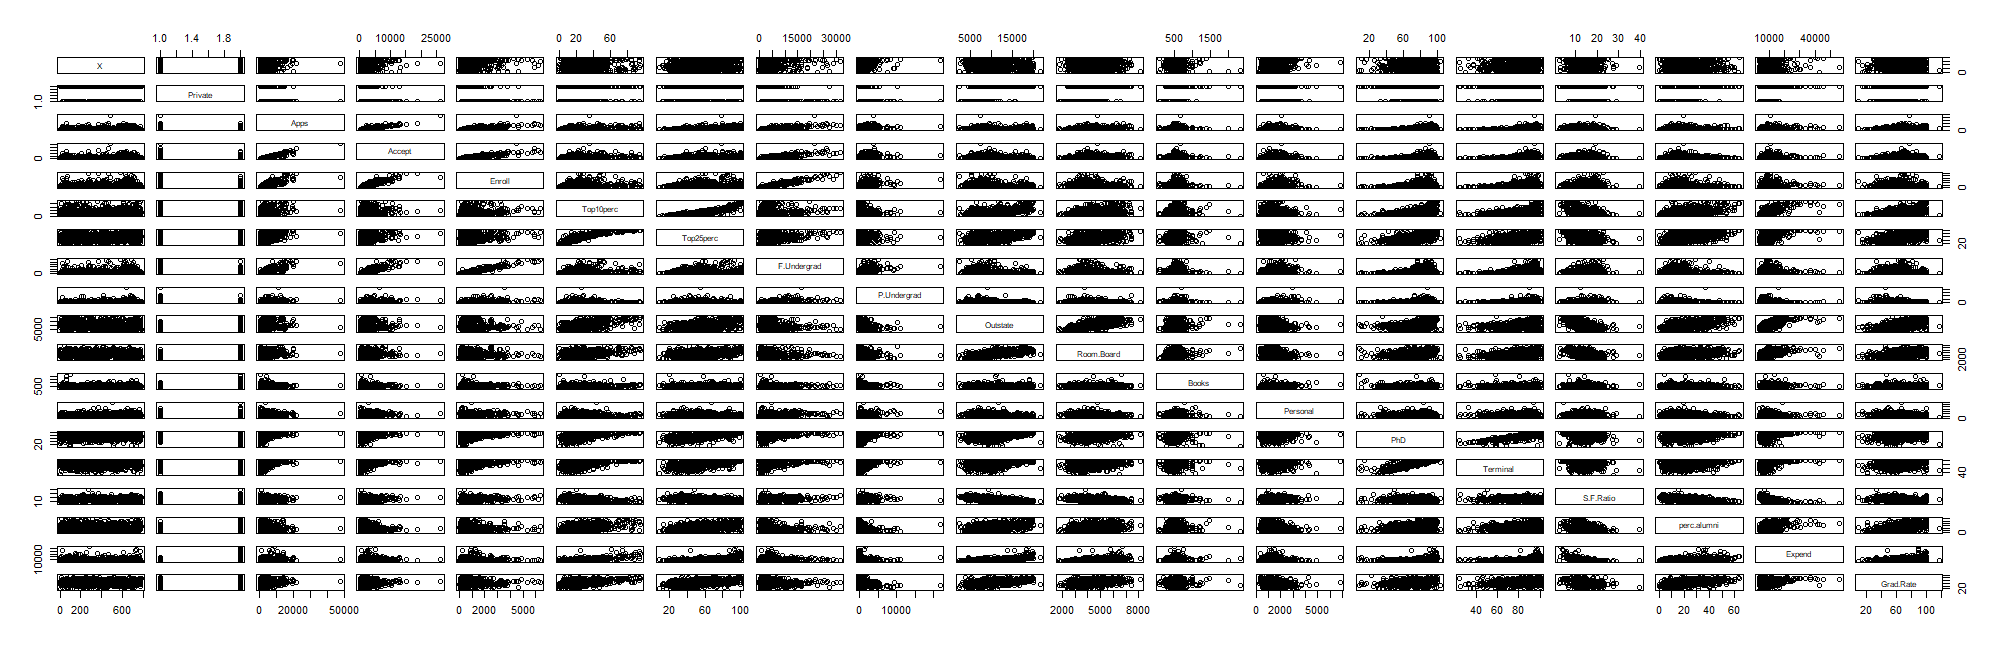
\includegraphics[width=1.3\linewidth]{Rplot}}\\[2ex]
iii.\\
\centerline{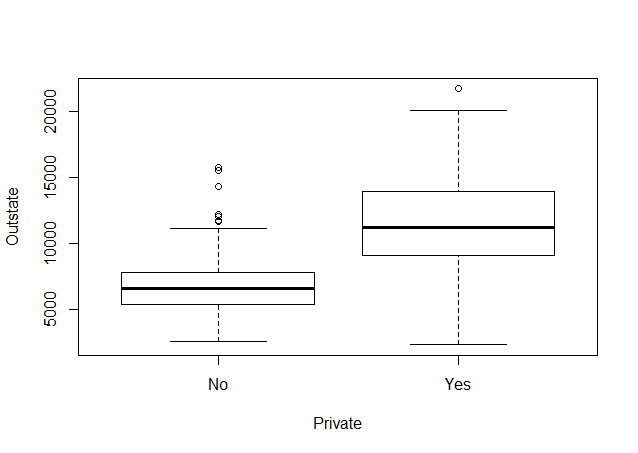
\includegraphics[width=1\linewidth]{box}}
iv.\begin{verbatim}
Elite=rep("No",nrow(college ))
Elite[college$Top10perc>50]="Yes"
Elite=as.factor(Elite)
college=data.frame(college,Elite)
summary(college)
\end{verbatim}
\centerline{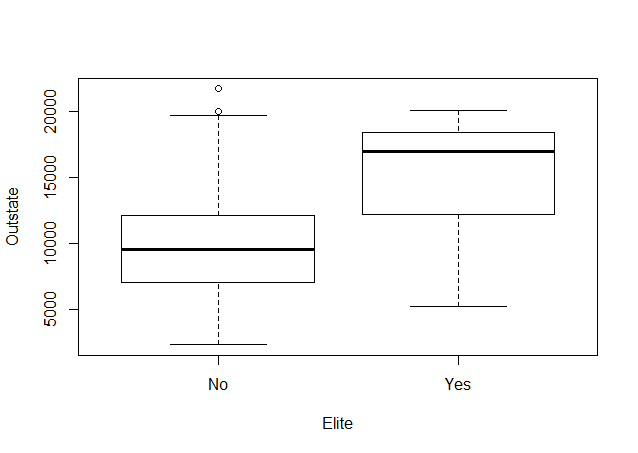
\includegraphics[width=0.8\linewidth]{box2}}
v.\\
\centerline{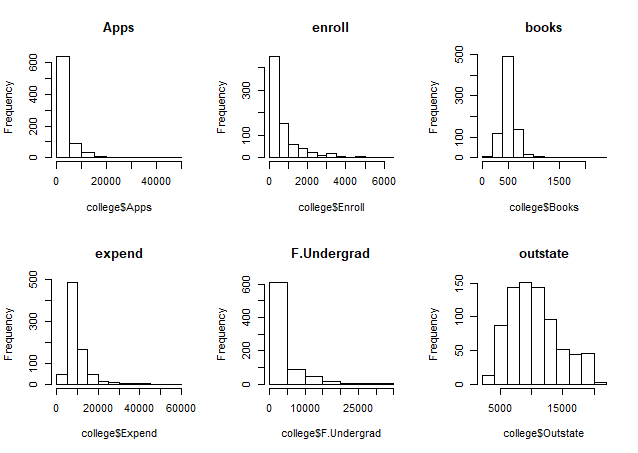
\includegraphics[width=0.9\linewidth]{hist}}\\[2ex]
vi.\\
\centerline{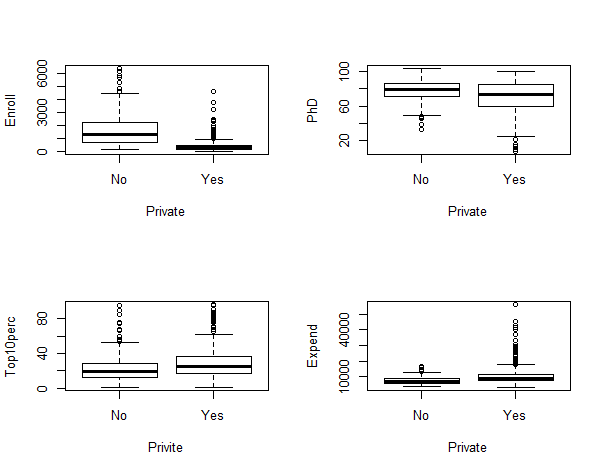
\includegraphics[width=1.0\linewidth]{explore}}\\[2ex]
\normalsize
\hspace{25pt}As shown in figure, we compare the schools which are private to public ones.We want to know which class of variance is larger, so we check four features of the dataset through coding.\\[2ex]
$$\begin{tabular}[c]{|c|c|c|c|c|}
\hline
 Class & Enroll & PhD & Top $10\%$ & Expend\\
\hline
Private & 209332.9 & 301.05 & 318.67 & 32291667\\
\hline
Public & 1591614.4 & 151.72 & 261.81 & 7265945\\
\hline
\end{tabular}$$
\ \\[2ex]
According to the result, the variance of private schools is larger than public ones except for Enroll.
\end{itemize}
\newpage
%%%%%%%%%%%%%%%%%%%%%%%%%%%%%%%%%%%%%%%%%%%%%%%%%%%%%%%%%%
9.
\begin{itemize}
\item[\small(a)]
\ \\
Quantitative : \small{mpg, displacment, horsepower, weight, acceleration}\\[3ex]
\Large{Qualitative} : \small{cylinders, year, origin, name}
\item[(b)]
\ \\
$$
\begin{tabular}[c]{|c|c|c|c|c|c|}
\hline
\ &mpg&displacement&horsepower&weight&acceleration\\
\hline
range&$9.0\thicksim46.60$ & $68.0\thicksim455.0$ & $46.0\thicksim230.0$ &$1613\thicksim5140$ & $8.00\thicksim24.80$\\
\hline
\end{tabular}
$$
\item[(c)]
$$
\begin{tabular}[c]{|c|c|c|c|c|c|}
\hline
statistics& mpg & displacement & horsepower & weight & acceleration \\
\hline
mean  &$23.45$ &$194.41$ &$104.47$ &$2977.58$ &$15.54$ \\
\hline
std  &$7.81$ &$104.64$  &$38.49$  &$849.40$ &$2.76$ \\
\hline
\end{tabular}$$
\item[(d)]
\raggedright
$$
\begin{tabular}{|c|c|c|c|c|c|}
\hline
statistics& mpg & displacement & horsepower & weight & acceleration\\
\hline
range &$11.00\thicksim46.60$&$68.0\thicksim455.0$&$46\thicksim230$&$1649\thicksim4997$&$8.50\thicksim24.80$\\
\hline
mean & $24.37$ & $5.38$ & $187.75$ & $100.96$ & $2939.64$\\
\hline
std & $7.88$ & $1.66$ & $99.94$ & $35.90$ & $812.65$\\
\hline
\end{tabular}$$
\item[(e)]
\ \\[0.5ex]
\centerline{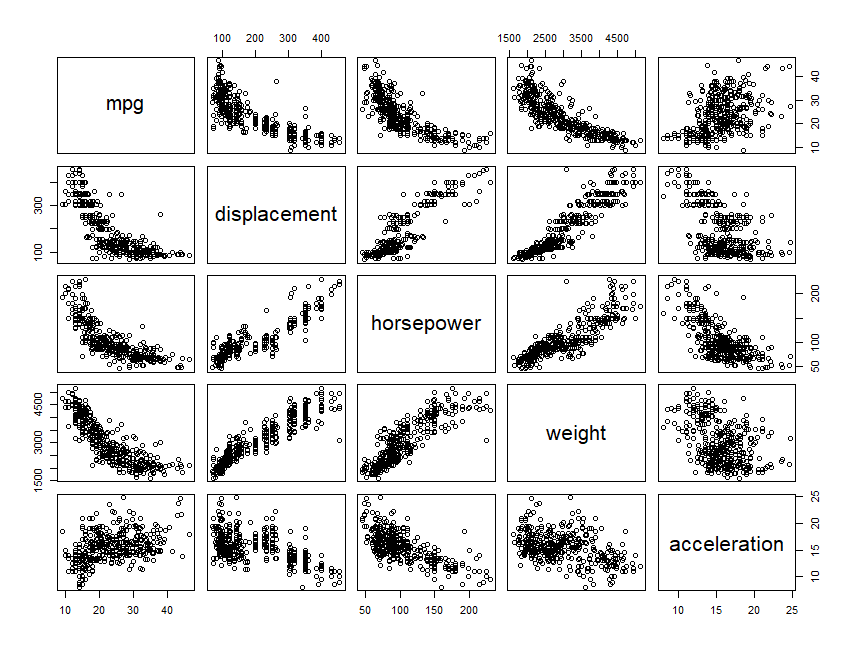
\includegraphics[width=0.6\linewidth]{correlation}}
\hspace{25pt}As shown in figure, we can see that mpg is negative correlated with many of predictors.
However, the acceleration is not highly correlated with mpg.\\
\item[(f)]
\ \\
\begin{verbatim}
> cor(auto$mpg,auto$weight)
[1] -0.8322442
> cor(auto$mpg,auto$horsepower)
[1] -0.7784268
> cor(auto$mpg,auto$displacement)
[1] -0.8051269
\end{verbatim}
We can use weight to predict mpg, because the correlation between weight and mpg is\ $-0.83$, that means they are highly correlated.
\end{itemize}
\newpage
%%%%%%%%%%%%%%%%%%%%%%%%%%%%%%%%%%%%%%%%%%%%%%%%%%%%%%%%%%
10.
\begin{itemize}
\item[\small(a)]
\ \\
\small 506 rows, 14 columns.\\[3ex]
The rows represent how many suburbs observed in this dataset. \\[3ex]
The columns represent the features of  the dataset.
\item[(b)]
\ \\
\centerline{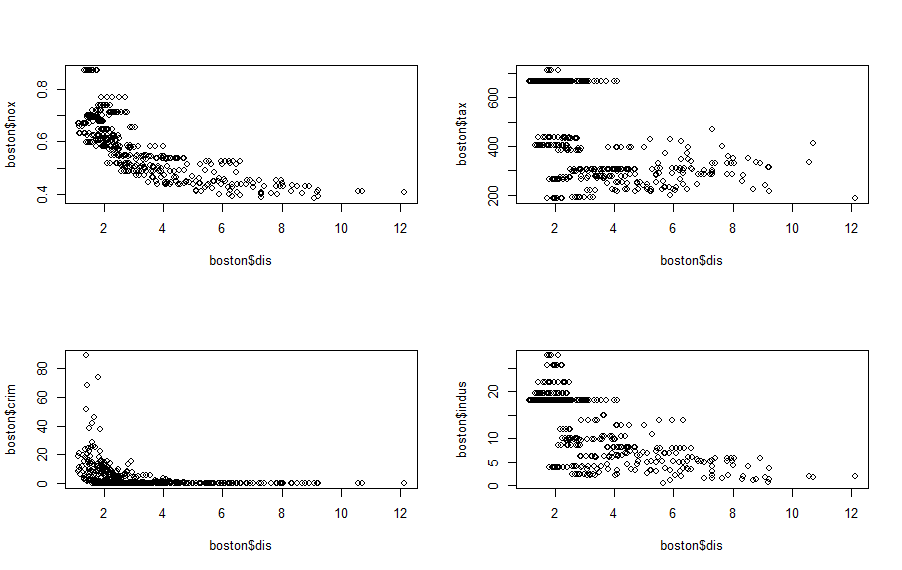
\includegraphics[width=1.15\linewidth]{four}}\\[4ex]
We want to know the predictors associated with distance, as shown in figure, only Nitrogen Oxides Concentration(nox) is negative correlated with distance.
\item[(c)]
\ \\[2ex]
The index of accessibility to radial highways(rad) is associated with per capita crime rate. Because it has the highest correlation coefficient between crim than any other predictor.\\[3ex]
\begin{verbatim}
for(i in 2:14)
{
 x[i-1]=cor(Boston$crim,Boston[,i])
}
> max(x)
[1] 0.6255051
> cor(Boston$crim,Boston$rad)
[1] 0.6255051
\end{verbatim}
\item[(d)]
\begin{verbatim}
summary(Boston)
\end{verbatim}
\ \\
Through coding, we can find that there are some suburbs appear to have particularly high crime rates and tax rates.
\item[(e)]
There are 35 suburbs in this data set bound the Charles river.
\begin{verbatim}
> summary(as.factor(Boston$chas))
  0   1
471  35
\end{verbatim}
\item[(f)]
$19.05$
\begin{verbatim}
> median(Boston$ptratio)
[1] 19.05
\end{verbatim}
\item[(g)]
\begin{verbatim}
summary(Boston)
min(Boston$medv)
\end{verbatim}
Through coding, we discover that the suburb has lowest median value of owner occupied is high in most of features.
\item[(h)]
$64$ suburbs average more than seven rooms per dwelling.\\[2ex]
$13$ suburbs average more than eight rooms per dwelling.
\begin{verbatim}
> bo=boston[which(boston$rm>7),]
> nrow(bo)
[1] 64
> bo=boston[which(boston$rm>8),]
> nrow(bo)
[1] 13
\end{verbatim}
The suburbs which average more than eight rooms per dwelling are high in black and low in dis, lstat and crime.
\end{itemize}
\end{document} 